\documentclass{beamer}
\usetheme{Madrid}
\usecolortheme{default}
%\usepackage[english]{babel}

\title{\textsc{Three Curves}}
\subtitle{Student ID:123456789}
\author{Your Name}
\institute{UNNC}
\date{\today}


\begin{document}
\begin{frame} % title slide
\titlepage
\end{frame}

\begin{frame}\frametitle{TABLE OF CONTENTS}\label{TO}
\tableofcontents
\end{frame}

\section{Three Curves}
\begin{frame}\frametitle{THREE FUNCTIONS}\label{TF}
\begin{columns}
\column<1->{0.5\textwidth}
\begin{eqnarray}
y & = & e^{x^3-1}\\
z & = & 2x e^{x^3-1}\\
w & = & x\sin(x)+1
\end{eqnarray}

\column<2->{0.5\textwidth}
\begin{figure}
\centering
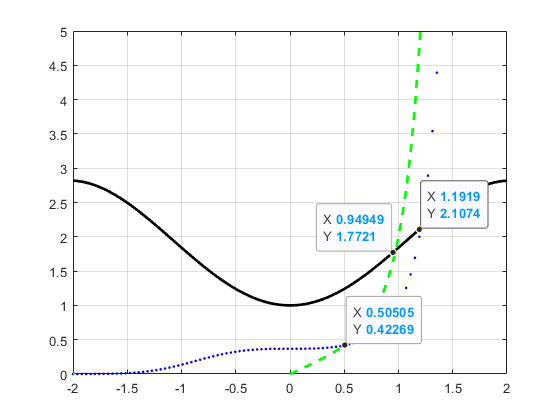
\includegraphics[scale=0.45]{threeCurves}
\caption{Three Curves}
\end{figure}
\end{columns}
\end{frame}

\section{Observations}
\begin{frame}\frametitle{OBSERVATIONS}\label{OBS}
\begin{table}[h]
\begin{tabular}{c|c|c|c}
Functions & Intersection with $f$ & Intersection with $g$ & Intersection with $h$\\
\hline
\hline
$f(x)$ & -- & $(0.50505,0.42269)$ & $(1.1919,2.1074)$\\
\hline
$g(x)$ & $(0.50505,0.42269)$ & -- & $(0.94949,1.7721)$\\
\hline
$h(x)$ & $(1.1919,2.1074)$ & $(0.94949,1.7721)$ & --\\
\hline
\end{tabular}
\end{table}
\end{frame}

\section{Links}
\begin{frame}\frametitle{Summary}
\hyperlink{OBS}{\beamergotobutton{GoTo Observations}}\\
\hyperlink{TF}{\beamerskipbutton{Skip to Three Functions}}\\
\hyperlink{TO}{\beamerreturnbutton{Return to Table of Contents}}
\end{frame}














\end{document}